
\part{Economics}
\label{ch:economics}

\begin{chapquote}{Lewis Carroll, \textit{Alice in Wonderland}}
``A large rose tree stood near the entrance of the garden: the roses on it were
white, but there were three gardeners at it, busily painting them red. This
Alice thought a very curious thing...''
\end{chapquote}

\textit{Money doesn’t grow on trees.} To believe that it does is foolish, and our
parents make sure that we know about that by repeating this saying like a
mantra. We are encouraged to use money wisely, to not spend it frivolously,
and to save it in good times to help us through the bad. Money, after all,
does not grow on trees.

Bitcoin taught me more about money than I ever thought I would need to know.
Through it, I was forced to explore the history of money, banking, various
schools of economic thought, and many other things. The quest to understand
Bitcoin lead me down a plethora of paths, some of which I try to explore in
this series.

In the first seven lessons some of the philosophical questions Bitcoin touches
on were discussed. The next seven lessons will take a closer look at money and
economics.

~

Part II -- Economics:

\begin{enumerate}
  \item Financial ignorance
  \item Inflation
  \item Value
  \item Money
  \item The history and downfall of money
  \item Fractional reserve insanity
  \item Sound money
\end{enumerate}

Again, I will only be able to scratch the surface. Bitcoin is not only
ambitious, but also broad and deep in scope, making it impossible to cover all
relevant topics in a single lesson, essay, article, or book. I  doubt if it is
even possible at all.

\textit{Bitcoin is a new form of money}, which makes learning about
economics paramount to understanding it. Dealing with the nature of human action
and the interactions of economic agents, economics is probably one of the
largest and fuzziest pieces of the Bitcoin puzzle.

Again, these lessons are an exploration of the various things I have learned
from Bitcoin. They are a personal reflection of my journey down the rabbit hole.
Having no background in economics, I am definitely out of my comfort zone and
especially aware that any understanding I might have is incomplete. I will do my
best to outline what I have learned, even at the risk of making a fool out of
myself. After all, I am still trying to answer the question: ``What have you
learned from Bitcoin?''

\begin{figure}
  \centering
  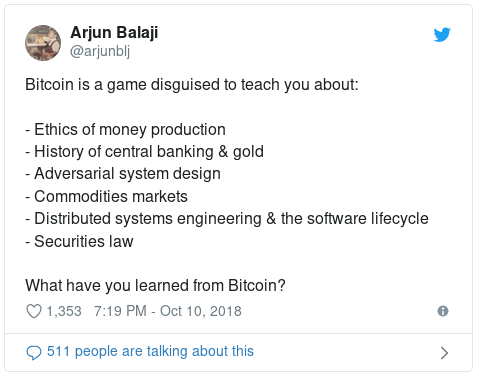
\includegraphics[width=8cm]{assets/images/the-tweet.png}
  \caption{What have you learned from Bitcoin?}
  \label{fig:the-tweet}
\end{figure}

After seven lessons examined through the lens of philosophy, let’s use the lens
of economics to look at seven more. Economy class is all I can offer this time.
Final destination: \textit{sound money}.

% [the question]: https://twitter.com/arjunblj/status/1050073234719293440
